\chapter{Evaluation} 

\label{Chapter5} % \ref{ChapterX}

%----------------------------------------------------------------------------------------
%	SECTION 1
%----------------------------------------------------------------------------------------

\section{Experimental Setup}

All versions of Autobahn were compiled using GHC
version \texttt{8.0.2}. The NoFib benchmarks were compiled with
GHC version \texttt{8.0.2} using NoFib's default flags, the flag
\texttt{-XBangPatterns}, and the NoFib flag that enables profiling.
We discarded the benchmarks in the NoFib suite that failed to compile
or run out of the box. We also excluded the benchmarks that \Ao{}
refuses to optimize because they already have very fast runtimes. That
left 60 benchmarks on which we could run experiments, listed in \figref{tab:nofib-list}.

\subsection{Runtime Performance Ratio}
To study runtime performance results, we report what we call
the \textit{runtime performance ratio}, which is the ratio of the
optimized program's runtime to the runtime of the original program. 
A runtime performance ratio of 1 indicates that
the optimized version of the program has the same runtime as the
original version and is therefore \textit{\unimp{}}.  A runtime
performance ratio of 2 is a sentinel value indicating that the
``optimized'' version of the program is \textit{\nonterm{}}, by which
we mean it runs for more than a timeout threshold longer than the
unoptimized program. 

\subsection{Successes and Failures}
A ratio that reflects a performance improvement of more than \absim{}
is considered successful because such a ratio indicates the
optimized program performs substantially better than the original, 
while ratios that improve less than \absim{} are failures. 
Failures can occur either as a result of \Ao{} failing to find 
performance improving bang placements or \At{} failing to eliminate 
bangs without significantly worsening runtime performance. 
Failures have the effect of leaving the program
unchanged as the proposed annotations are discarded in favor of the
original (or in favor of the \Ao{} optimized version, if the failure is due to \At{}).
When we study the results of a particular optimization system on a
particular benchmark, we also categorize the results into one of three
groups: complete success, partial success, and complete failure.  A
benchmark completely succeeds if all of its 10 runs are successful,
completely fails if all of its runs are failures, and partially
succeeds if there is a mixture of these outcomes.

\subsection{Approach}
To calculate the performance of a particular benchmark using a
particular optimization system (\eg{}, \At{} or a
restricted version using only a subset \At's phases), we ran the system under test on the benchmark 10
times to account for random fluctuations. We also test the performance of the benchmark on \At{} using both runtime and memory allocations as the \profm{}. We scored each run by its runtime performance
ratio. Note that each run of the benchmark can produce a different
result not only because of variations in machine load but also
because the search process is randomized.  Failed runs can be further
categorized into runs in which \Ao{} fails and runs in which
the \postopt{} phase of \At{}
fails. If a benchmark failed at the \Ao{} stage, then we say that its
runtime performance ratio for that run is 1 and it recommended
0~bangs. If a benchmark succeeded at the \Ao{} stage but failed
in the \postopt{} phase, then we say its runtime performance ratio is
1 (because we discard the optimization results) and the
number of inferred bangs is 0~bangs, because we discard the optimization annotations.  
Finally, we computed the \cut{\ksf{harmonic}}average of the runtime
performance ratios and the \cut{\ksf{arithmetic}}average of the number of
recommended bangs.

\begin{table}[!htb]
    \begin{minipage}{.5\linewidth}
      \centering
        \begin{tabular}{lllr}
            \hline
            Program    &   Loc    &   Files   &   Genes\\
            \hline
            callback002 &   41  &   1   &   3\\ 
            rfib        &   12  &   1   &   5\\
            threads007  &   16  &   1   &   5\\
            x2n1        &   35  &   1   &   6\\
            threads001  &   15  &   1   &   8\\
            callback001 &   41  &   1   &   9\\ 
            tak         &   16  &   1   &   9\\
            mutstore2   &   22  &   2   &   10\\
            spellcheck  &   13  &   1   &   10\\
            threads003  &   20  &   1   &   11\\
            mutstore1   &   25  &   2   &   12\\
            primes      &   18  &   1   &   12\\
            queens      &   19  &   1   &   18\\
            bernouilli  &   40  &   1   &   19\\
            kahan       &   58  &   1   &   23\\
            exp38       &   93  &   1   &   24\\
            pidigits    &   22  &   1   &   27\\
            integrate   &   43  &   1   &   28\\
            cryptarithm1&   164 &   1   &   33\\
            wheel-sieve1&   41  &   1   &   38\\
            fasta       &   58  &   1   &   44\\
            integer     &   68  &   1   &   47\\
            wheel-sieve2&   47  &   1   &   47\\
            life        &   53  &   1   &   48\\
            rsa         &   74  &   2   &   50\\
            binary-trees&   74  &   1   &   51\\
            maillist    &   178 &   1   &   52\\
            gcd         &   60  &   1   &   57\\
            cryptarithm2&   128 &   1   &   60\\
            lcss        &   60  &   1   &   71\\ 
        \end{tabular}
    \end{minipage}%
    \begin{minipage}{.5\linewidth}
      \centering
        \begin{tabular}{lllr}
            \hline
            Program    &   Loc    &   Files   &   Genes\\
            \hline
            atom        &   188 &   1   &   74\\
            paraffins   &   91  &   1   &   75\\
            calendar    &   140 &   1   &   92\\
            awards      &   115 &   2   &   99\\
            fish        &   128 &   1   &   102\\
            puzzle      &   170 &   1   &   103\\
            treejoin    &   121 &   1   &   119\\
            eliza       &   267 &   1   &   138\\
            sorting     &   131 &   2   &   196\\
            cichelli    &   195 &   4   &   205\\
            cse         &   464 &   2   &   222\\
            pic         &   527 &   9   &   235\\
            clausify    &   184 &   1   &   246\\
            minimax     &   238 &   6   &   299\\
            boyer2      &   723 &   5   &   302\\
            expert      &   525 &   6   &   424\\
            hidden      &   507 &   14  &   430\\
            gamteb      &   701 &   13  &   458\\
            prolog      &   643 &   9   &   514\\
            infer       &   600 &   16  &   586\\
            fem         &   1286&   17  &   655\\
            scs         &   585 &   7   &   770\\
            simple      &   1129&   1   &   845\\
            reptile     &   1522&   13  &   895\\
            symalg      &   1024&   11  &   1137\\
            gg          &   812 &   9   &   1192\\
            cacheprof   &   2151&   3   &   1228\\
            fulsom      &   1392&   13  &   1433\\
            fluid       &   2401&   18  &   1688\\
            anna        &   9561&   32  &   7709\\
        \end{tabular}
    \end{minipage} 
    \caption{Statistics for the NoFib benchmarks, sorted in increasing order of number of genes}
\label{tab:nofib-list}
\end{table}

%----------------------------------------------------------------------------------------
%	SECTION 2
%----------------------------------------------------------------------------------------

\section{\Preopt{} Search Space Reduction}

To assess the impact of the \preopt{} phase, we study the number of
genes that the phase eliminated from (or added to) consideration by \Ao{}.
We compare the number of bangs that \Ao{} inferred when run with and
without the \preopt{} phase, calling the optimizer comprised of
the \preopt{} phase plus \Ao{} the \textit{\Preopt{} optimizer.} We
note in how many of the runs the \Preopt{} optimizer failed.  Finally,
we compare the runtime performance ratio for \Ao{} with the ratio for
the \Preopt{} optimizer.
To compute this data, we ran both the \Preopt{} optimizer and \Ao{} on
the 60 programs from NoFib benchmark suite.  We optimized all runs 
using runtime as the profiling metric only, and we set both 
the \hotspotcost{} and \absim{} thresholds to 6\%.

The \preopt{} phase eliminated at least one file in 21 out of the 60 
benchmark programs.
The remaining 39 benchmarks fall into one of two categories.
The first category consists of 33 benchmarks that did not have any files
eliminated by the \preopt{} phase. The second category comprises
6 benchmarks that the \preopt{} phase determined were not suitable for
optimization because they had no significant \hotspots{}.
Since \Ao{} and the \Preopt{} optimizer handle these 39 benchmarks
identically, we exclude them from the graphs reporting on the results
of the \preopt{} phase. We discuss the second category of benchmarks in
\secref{sec:file-elim}. None of the 60 programs in the benchmark suite
had an external \hotspot{} not in the original optimization coverage.

\figref{fig:preopt-bangs} shows the results from the 21 benchmarks that
had at least one file eliminated during the \preopt{} phase. The
column \texttt{Eliminated Genes} gives the number of potential bang
locations that were eliminated before \Ao{} ran.
The \texttt{Original Bangs} column records the number of bangs in the
original program, most of which were zero.
The \texttt{Failed runs} column gives the fraction of the 10 runs on
which the \Preopt{} optimizer failed.
Finally, the \texttt{\Ao{} Bangs} and \texttt{\Preopt{} Bangs} columns
give the number of recommended bangs by the two systems,
respectively.  On average, the \preopt{} phase eliminated
\preoptElim{} genes per 100 LOC across the 60 programs in the benchmark suite before
invoking \Ao{}.
The \Preopt{} optimizer recommended \preoptFewerBangs{} fewer bangs
than \Ao{}.

The \texttt{anna}, \texttt{expert}, and \texttt{symalg} benchmarks are
particularly interesting because \Ao{} consistently failed to find
winning chromosomes for them, and so it did not generate any bangs. However,
after reducing the size of the search space, the \Preopt{}
optimizer was able to find meaningful bangs for them.

\figref{fig:preopt-runtime} shows the corresponding runtime
performance ratios produced by \Ao{} and the \Preopt{} optimizer on
the same 21 benchmarks.
The graph shows that even when a large number of genes are
eliminated prior to running the genetic algorithm, the optimizer is still able to
find \useful{} bangs that result in similar runtime improvement. This data
confirms that the eliminated genes were on the whole not \useful{}.
On average on these 21~programs, the \Preopt{} optimizer returns
runtime performance ratios of \preoptPerformance{} compared
to \AoPerformance{} for \Ao, which is an
optimization \textit{improvement}.


\begin{figure*}
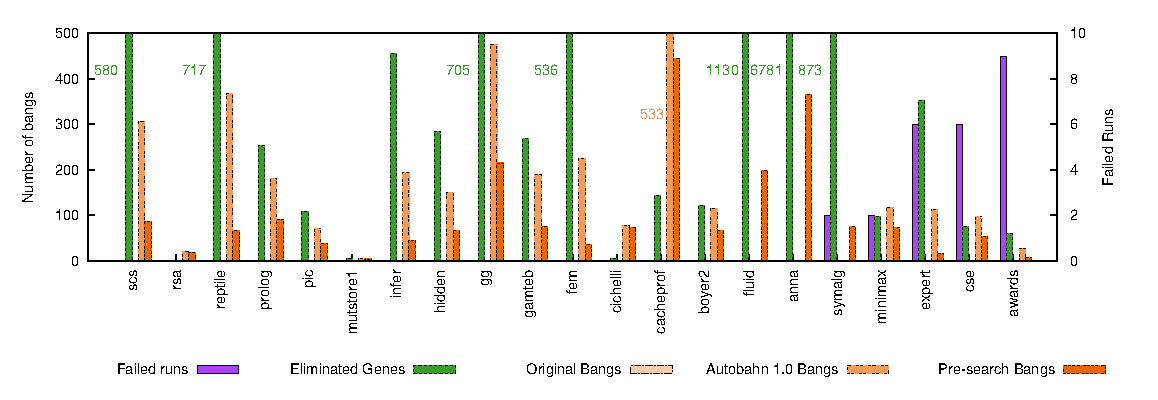
\includegraphics[width=\textwidth]{pre-aut-bangs}
\scaption{Number of bangs generated by \Ao{} vs. \Preopt{} optimizer across 21 benchmarks that had at least
one file eliminated during the \preopt{} phase. Columns that exceed
the maximum axis value are labeled with their actual values. The
benchmarks are sorted in increasing order of number of failed runs for
the \Preopt{} optimizer.}
\label{fig:preopt-bangs}
\end{figure*}

\begin{figure*}
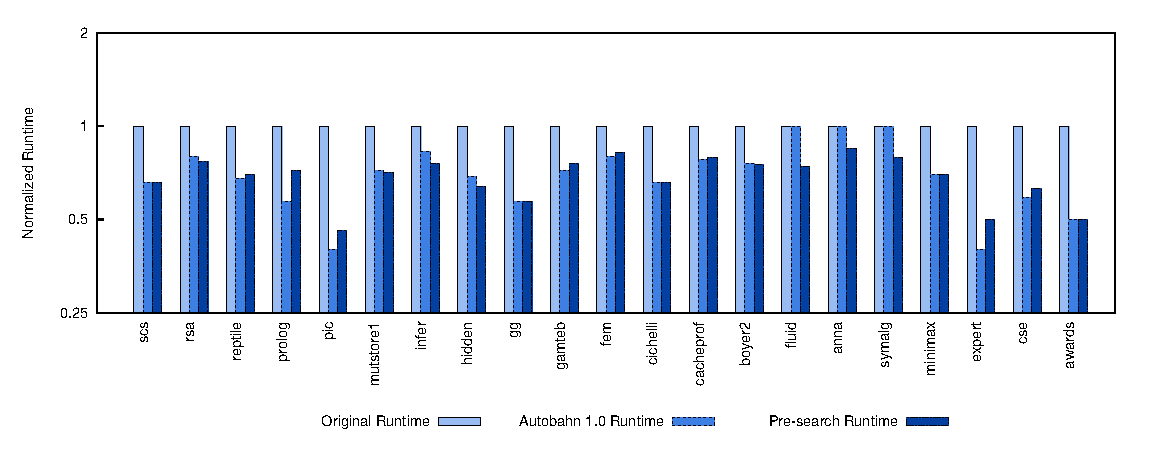
\includegraphics[width=\textwidth]{pre-aut}
\scaption{Performance runtime ratios of \Ao{} vs. \Preopt{} optimizer
across 21 benchmarks that had at least one
file eliminated during the \preopt{} phase. The x-axis
is on a base-2 log scale. The benchmarks appear in the same order as
in \figref{fig:preopt-bangs}.}
\label{fig:preopt-runtime}
\end{figure*}

%----------------------------------------------------------------------------------------
%   SECTION 3
%----------------------------------------------------------------------------------------

\section{\Preopt{} File Elimination}

\label{sec:file-elim}

The \preopt{} phase identifies 6 benchmarks among the 60 in our suite
as unsuitable for optimization when the \hotspotcost{}
threshold is set to 6\%:  \texttt{awards}, \texttt{callback001},
\texttt{callback002}, \texttt{mutstore2}, \texttt{sorting}, and \texttt{threads007}. As
expected, when attempting to
optimize \texttt{awards}, \texttt{sorting},
and \texttt{threads007}, \Ao{} consistently fails, returning
the \unimp{} runtime code. However, \Ao{} was able to
successfully optimize the other programs. Through inspection, we
concluded that \texttt{callback002} would have benefited from a
lower \hotspotcost{} threshold as its most costly hot spot takes up
3.9\% of the program runtime. Both \texttt{callback001}
and \texttt{threads007} would have benefited from inspecting heap
profiles instead of time and allocation profiles as the costs
associated with their hot spots were noticeably larger in heap
allocations while remaining insignificant in runtime
costs. The \texttt{mutstore2} program's performance fluctuated wildly
even without bangs in it. For example, its measured runtime was as low
as 60\% - 80\% of its original runtime in one-third of the experiments
we ran with no bangs in the program. Therefore, the optimization
results were likely skewed by the fluctuating runtime.

%----------------------------------------------------------------------------------------
%   SECTION 4
%----------------------------------------------------------------------------------------

\section{\Preopt{} File Addition}

To demonstrate the effectiveness of using the \preopt{} phase to
expand Autobahn's coverage for improved optimization results, we
tested our approach on the \texttt{sumList} microbenchmark. We
created \texttt{sumList} to simulate the scenario in which a
programmer references code from an external library or external file
that contains \hotspots{} but is not within the current optimization
coverage.

The \texttt{sumList} program's \texttt{Main.hs} file contains only one
function: a main function that constructs a list of integers from 1 to
1,000,000 and then calculates the sum of all integers in the list using an
external \textit{sum} function located in \texttt{Sum.hs}. Users
may decide to set the optimization coverage to [\texttt{Main.hs}],
because they are interested in making the main program run
faster. However, as demonstrated in \figref{fig:sumList}, \Ao{} was only able to
improve program performance by 3\%, even when it was able to
exhaustively search the possible bang locations in the 6 lines of code in the \texttt{main}
function. Upon inspecting the results, users may be mistaken in
believing that their program runtime cannot be improved
further.

But there are indeed other opportunities to speed up \textit{sumList}
located in places that the users did not think about. If the users were
to rerun the optimization using the \preopt{} phase, then GHC's time and
allocation profile indicates that the largest \hotspotcost{} was 9.5\%
and located in lines 7 to 8 in the \textit{sum} function
in \texttt{Sum.hs}. The \textit{sum} function is entirely lazy and did
not immediately compute the sum of each integer as it recursed through
the list. In the resulting log file, the \preopt{} phase
suggests
adding \texttt{Sum.hs} to the optimization coverage.
After expanding the coverage and re-running the optimization,
the resulting \texttt{sumList} ran at only 13\% of the original
runtime, a dramatic improvement.

Although the \texttt{sumList} example is short and synthetic, it shows
the larger potential for users to obtain much better optimization
results when running the \preopt{} phase in conjunction
with \Ao{}. Programmers often build upon each other's code and use
external functions that they may not be entirely familiar with or did
not consider optimizing. The \preopt{} phase can identify valuable
missed opportunities. Of
course, the addition of more files to optimize means that more bangs
might be generated. It is up to the user to decide if they want to add
the suggested files for better optimization results at the risk of
needing to inspect more bangs.
\newline

\begin{figure}
\centering
\begin{tabular}{p{3cm}p{3.5cm}p{4cm}p{1.5cm}}
\hline
Version   & Coverage & Normalized Runtime & No.Bangs \\
\hline
Original      & N/A   &   1  & 0   \\
\Ao{}       & [\texttt{Main.hs}]      & 0.97    &  2\\
Pre-optimization    & [\texttt{Main.hs}, \texttt{Sum.hs}]         & 0.13      & 4\\
\hline
\end{tabular}
\scaption{Results for \texttt{sumList} microbenchmark.}
\label{fig:sumList}
\end{figure}

%----------------------------------------------------------------------------------------
%   SECTION 5
%----------------------------------------------------------------------------------------

\section{\Postopt{} Bang Reduction}

To assess the effectiveness of the \postopt{} phase,
we compare the results of running \Ao{} with running
the \textit{\Postopt{} optimizer} comprised of \Ao{} followed by
the \postopt{} phase.
\cut{
Already discussed and so not necessary:
Similarly, we took the mean of running the
program ten times on the NoFib benchmark suite while optimizing on
runtime only, and set both \hotspotcost{} and \absim{} thresholds to
6\%.
A benchmark is successfully optimized if \Ao{} improved its
performance by at least 6\% after optimization. }
Figures~\ref{fig:post-bangs-all} and \ref{fig:post-ratio-all}
give the number of bangs and the runtime performance ratios,
respectively, for the 21 benchmarks that \At{} successfully optimized on all 10 runs.
Figures~\ref{fig:post-bangs-some} and \ref{fig:post-ratio-some}
give the number of bangs and the runtime performance ratios, respectively,
for the 28 benchmarks on which \At{} was partially successful,
sorted in increasing order of \At{}'s failure rate.
We do not show the results from the remaining 12 benchmarks that \At{}
failed to optimize on every run since the numbers for those benchmarks
would be unchanged from the original program.  \figref{fig:post-failures} shows how
frequently a benchmark failed at the \Ao{} stage vs. how frequently it
failed at the \postopt{} phase. The graph shows that the majority of \Postopt{} optimizer fails are
caused by failures at the \Ao{} stage, which produces a poorly
performing set of bangs for the \postopt{} phase to
minimize. Therefore, benchmarks that failed at the \Ao{} stage are
highly likely to fail during  the \postopt{} phase as well.


Figures~\ref{fig:post-bangs-all} and \ref{fig:post-bangs-some} show
that the number of bangs eliminated by the \Postopt{} optimizer is quite
significant: on average \postBangs{}. Figures~\ref{fig:post-ratio-all}
and~\ref{fig:post-ratio-some} show the corresponding runtime
performance ratios of each optimized program. In most benchmarks,
the \Postopt{} optimizer does
a little worse than \Ao{}, on average \postRatioWorse{} worse, because
the \postopt{} phase only preserves bangs that affect program
runtime by at least the \absim{} threshold (6\% in these experiments).
If users want to
maintain higher levels of optimization,
they can lower the \absim{} threshold so the minimizer becomes less
aggressive in bang elimination. That way, more bangs will be
preserved, but runtime performance will
improve.

Looking at these results in more detail,
the \texttt{callback001} and \texttt{pic} benchmarks are good
examples of when a program has no cost centers that meet
the \hotspotcost{} threshold, so the \postopt{} phase eliminated all their bangs.
In these cases, a lower threshold would have
helped discover useful bangs that are located in the relatively colder locations.
The data for \texttt{anna} and \texttt{fluid}
show that while \Ao{} found bangs that triggered a \nonterm{} runtime
code, \postopt{} bang elimination was able to eliminate
the \dangerous{} bangs that caused the bad behavior and instead produce
successful optimization results.

\begin{figure*}
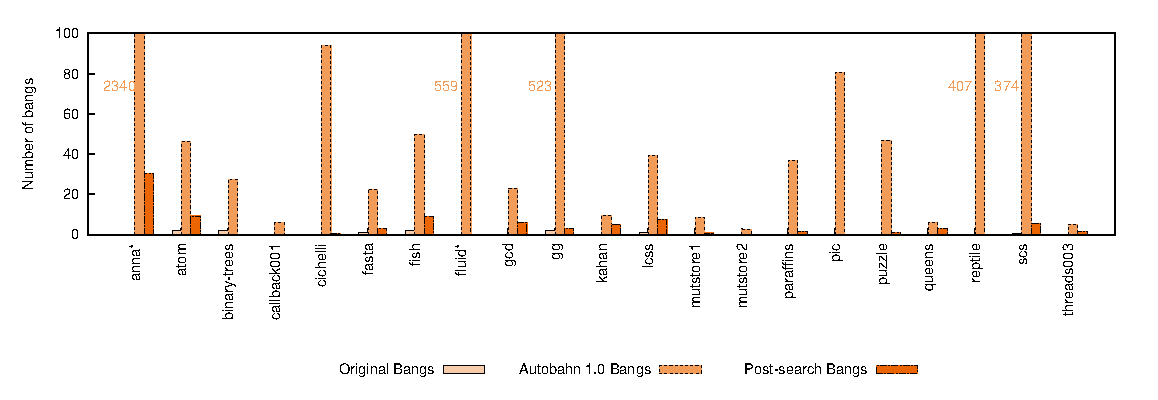
\includegraphics[width=\textwidth]{aut-post-bangs}
\scaption{Number of bangs generated by \Ao{} vs. \Postopt{} optimizer
across 21 benchmarks that \At{} successfully optimized
every time. Columns that exceed the maximum axis value are labeled
with their actual values. }
\label{fig:post-bangs-all}
\end{figure*}

\begin{figure*}
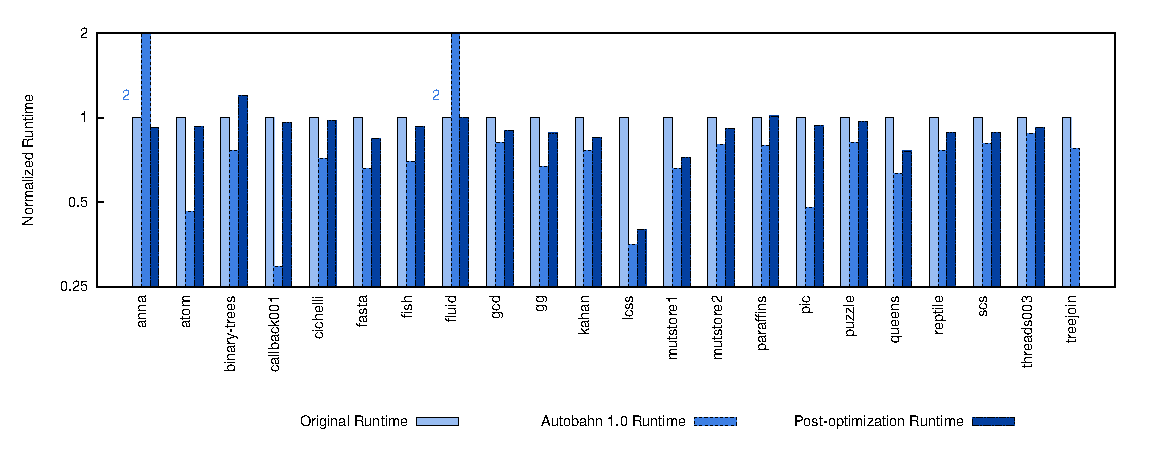
\includegraphics[width=\textwidth]{aut-post}
\scaption{Performance runtime ratios of \Ao{} vs. \Postopt{} optimizer
across 21 benchmarks that \At{} successfully
optimized every time. The x-axis is on a base-2 log scale.
For the *-ed benchmarks, \Ao{} generated non-terminating
optimization results, but the \postopt{} phase removed
the \dangerous{} bangs and succeeded in optimizing the program. }
\label{fig:post-ratio-all}
\end{figure*}

\begin{figure*}
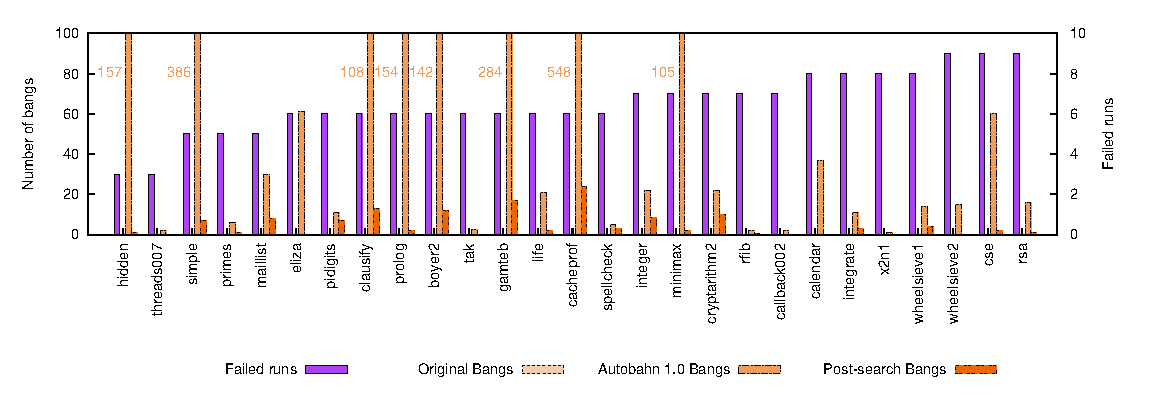
\includegraphics[width=\textwidth]{ap-partial-bangs}
\scaption{Number of bangs generated by \Ao{} vs. \Postopt{} optimizer
across 27 benchmarks that \At{} successfully optimized on some runs. Failure rate
out of 10 runs is shown. Columns that exceed
the maximum axis value are labeled with their actual values.
The benchmarks are sorted in increasing order of \At{} failure rate. }
\label{fig:post-bangs-some}
\end{figure*}

\begin{figure*}
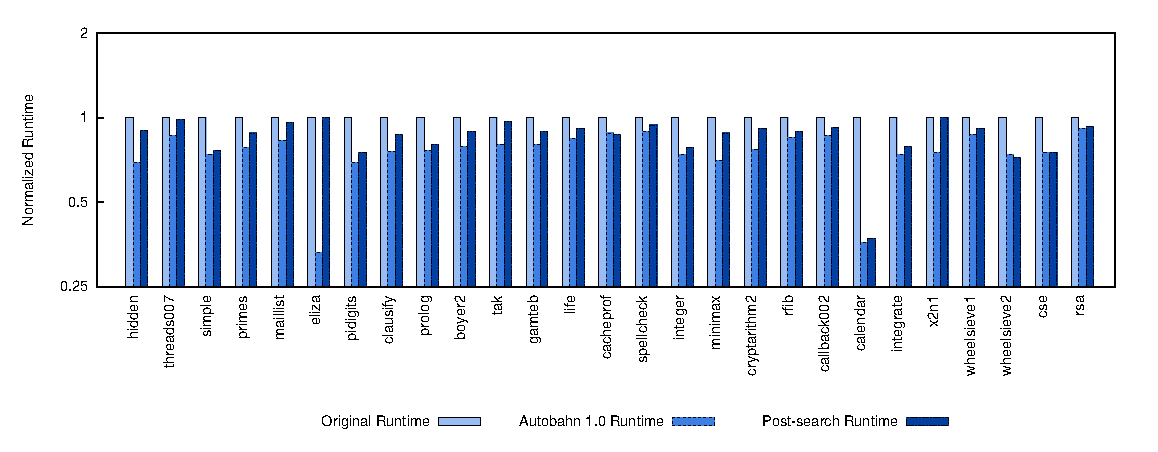
\includegraphics[width=\textwidth]{ap-partial}
\scaption{Performance runtime ratios of \Ao{} vs. \Postopt{} optimizer
across 27 benchmarks that \At{} successfully optimized on some runs.
The x-axis is on a base-2 log scale.
}
\label{fig:post-ratio-some}
\end{figure*}

\begin{figure*}
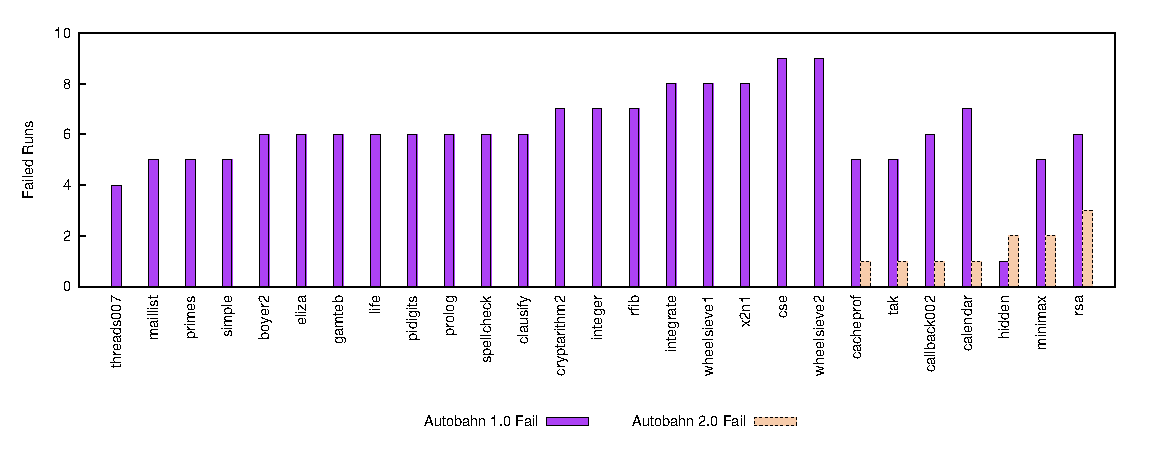
\includegraphics[width=\textwidth]{aut-post-fail}
\scaption{Frequency of failures attributable to \Ao{} vs
the \postopt{} phase across 27
benchmarks on which optimization sometimes succeeded. Benchmarks are sorted in
increasing order of \Postopt{} optimizer failure rate. }
\label{fig:post-failures}
\end{figure*}

%----------------------------------------------------------------------------------------
%   SECTION 6 
%----------------------------------------------------------------------------------------

\section{\At{}: Combining \preopt{} and \postopt{}}

To evaluate the overall effectiveness of \At{}, we ran the complete
tool chain on our NoFib benchmarks 10 times. Figures~\ref{fig:2-bangs-26}, \ref{fig:2-ratio-26}, \ref{fig:2-bangs-52},
and \ref{fig:2-ratio-52} presents the numbers of recommended bangs and
the runtime performance ratios on the 52 benchmarks that \At{}
successfully optimized at least once using runtime as the \profm{}.
All benchmarks are sorted in increasing order of \At{} failure rate.

Out of those 60 programs, the \preopt{} phase eliminated 5 because they had no \hotspots{}.  
On another 3 benchmarks, neither \Ao{} nor \At{}
successfully found an optimization on any run.
It is interesting to note that only these 8
benchmarks consistently failed under \At{}, while 12
consistently failed under the \Postopt{} optimizer.
This observation shows that the \preopt{} phase successfully
increased the effectiveness of the later optimization phases.

Overall, \At{} reduced the number of bangs generated by 90.2\%
with an optimization degradation of 15.7\%.
We split the data into two graphs of 26 benchmarks each for bang counts
(Figures~\ref{fig:2-bangs-26} and~\ref{fig:2-bangs-52})
and for runtime performance ratios
(Figures~\ref{fig:2-ratio-26} and~\ref{fig:2-ratio-52})
for legibility.
Finally, \figref{fig:2-failures} shows how frequently a benchmark
failed at the \Ao{} stage versus at the end of \At{}. As with
the \postopt{} optimizer, the majority of runs failed at the \Ao{} stage.


While most benchmarks consistently showed significant bang reduction
with minimal optimization degradation under \At{}, a few benchmarks stand
out. The \texttt{expert} and \texttt{calendar} benchmark not only had
bangs reduced by 79.41\% and 97.63\% respectively, but also
experienced performance \textit{improvements} of 27.60\% and 14.82\%
respectively. It is worth noting that both benchmarks failed
more times than they succeeded, so such results are not guaranteed to
be replicable in every run. The \texttt{atom} benchmark is also noteworthy
because the \postopt{} phase eliminated all bangs
generated by \Ao{}, yet it still had a runtime performance ratio of
0.78. This finding suggests that \texttt{atom}'s original
runtime fluctuates by a significant amount on its own. It also
suggests that \texttt{atom}'s overall performance
improvement is achieved through the accumulation of speedups at many
relatively cold cost centers, so lowering \At{}'s \hotspotcost{}
might result in a better performance improvement.

\begin{figure*}
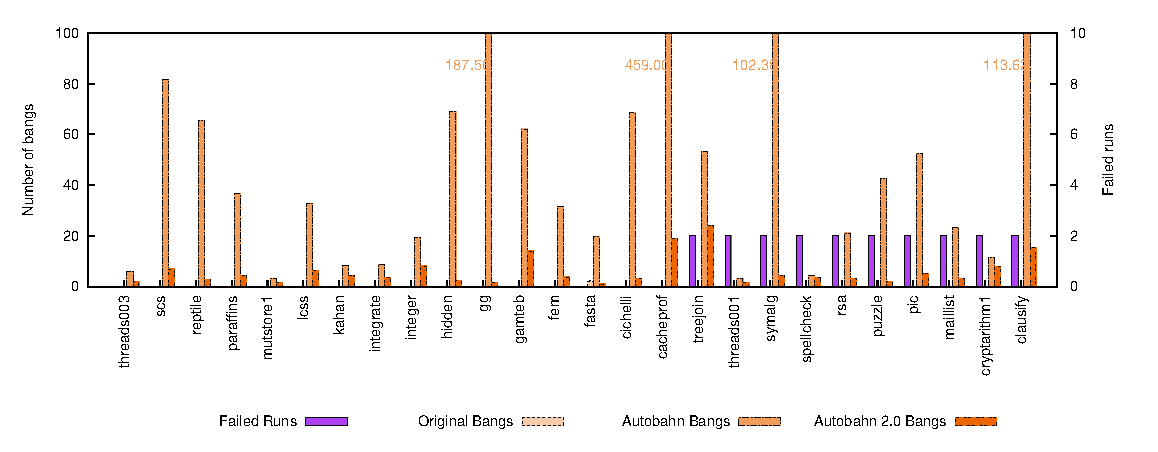
\includegraphics[width=\textwidth]{pap0-bangs}
\scaption{Number of bangs generated by \Ao{} vs. \At{} across the first
26 of 52 benchmarks that \At{} successfully optimized
at least once using runtime as the \profm{}. Failure
rate out of 10 runs is shown. Benchmarks are sorted in increasing order of
failure rate. Columns that exceed the maximum axis value are labeled
with their actual values.}
\label{fig:2-bangs-26}
\end{figure*}

\begin{figure*}
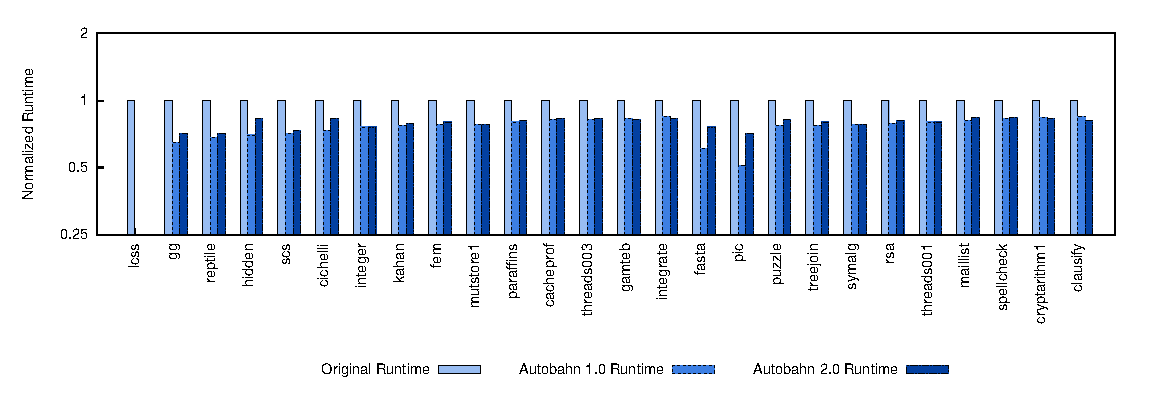
\includegraphics[width=\textwidth]{pap0}
\scaption{Runtime performance ratios of \Ao{} vs. \At{} across
the first 26 of 52 benchmarks that \At{} successfully optimized at least
once using runtime as the \profm{}. The x-axis is on a base-2 log scale.}
\label{fig:2-ratio-26}
\end{figure*}

\begin{figure*}
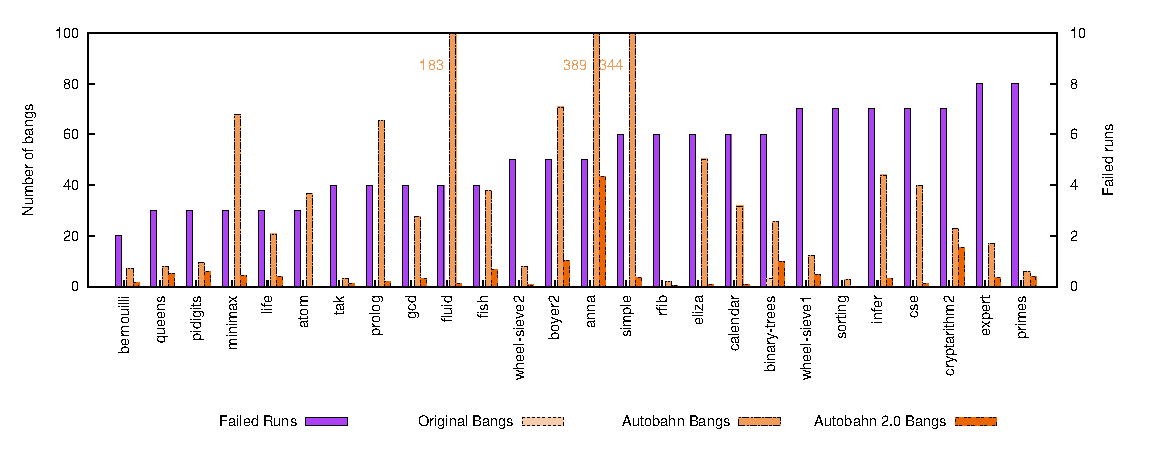
\includegraphics[width=\textwidth]{pap1-bangs}
\scaption{Number of bangs generated by \Ao{} vs. \At{} across the
remaining 26 of 52 benchmarks that \At{} successfully optimized at least
once using runtime as the \profm{}. Failure rate out of 10 runs is shown. 
Benchmarks are sorted in
increasing order of failure rate. Columns that exceed the maximum axis
value are labeled with their actual values. }
\label{fig:2-bangs-52}
\end{figure*}

\begin{figure*}
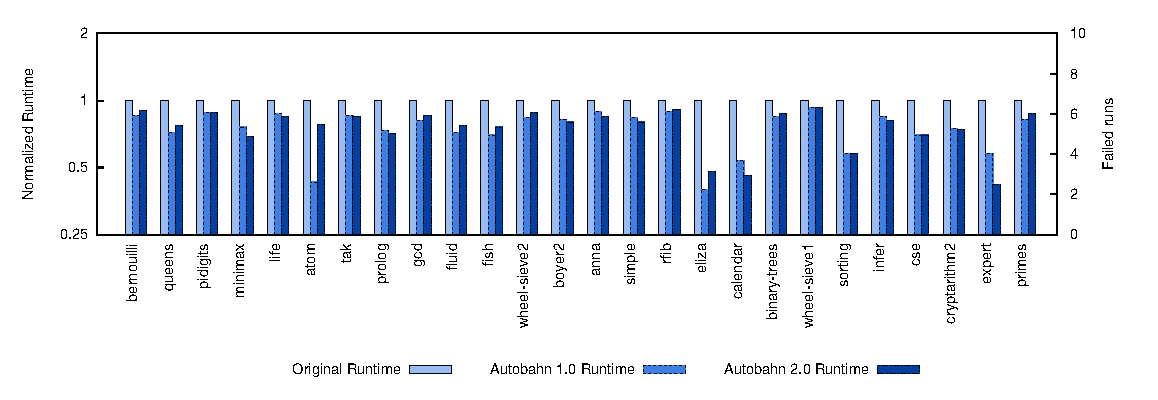
\includegraphics[width=\textwidth]{pap1}
\scaption{Runtime performance ratios of \Ao{} vs. \At{} across the
remaining 26 of 52 benchmarks that \At{} successfully optimized at least
once using runtime as the \profm{}. The x-axis is on a base-2 log scale.
}
\label{fig:2-ratio-52}
\end{figure*}

\begin{figure*}
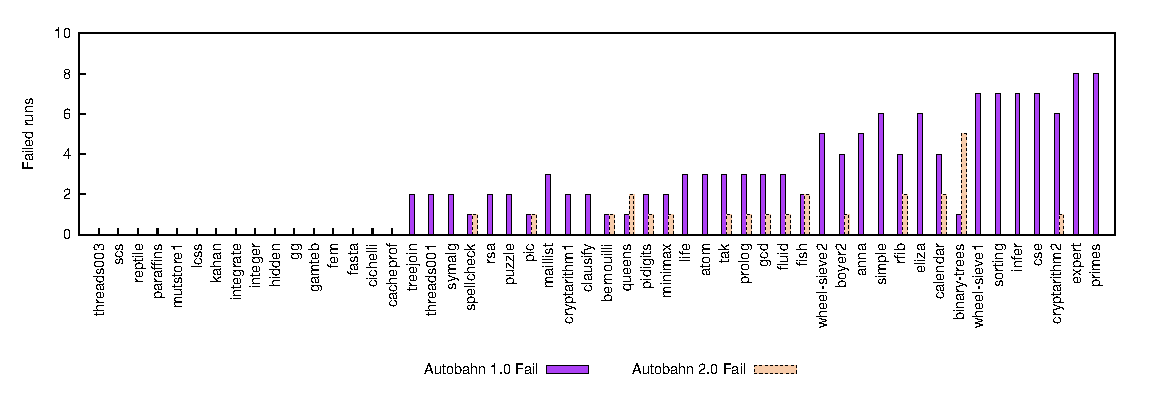
\includegraphics[width=\textwidth]{pap-fail}
\scaption{Frequency of failure attributable to \Ao{} versus \At{} across the 36
benchmarks that \At{} sometimes successfully optimized using runtime as the \profm{}. 
Benchmarks are sorted in increasing order of \At{} failure rate. }
\label{fig:2-failures}
\end{figure*}

\subsection{Runtime vs. memory allocations as \profm{}}

To evaluate whether there is a measurable performance difference in using 
memory allocations over runtime as the \profm{}, we also ran \At{} on the 
60 benchmarks 10 times (NOTE: will change this to 10 times when I finish running
all of them) using memory allocations as the \profm{}. 
Figures~\ref{fig:2-bangs-26-HA}, \ref{fig:2-ratio-26-HA}, \ref{fig:2-bangs-52-HA},
and \ref{fig:2-ratio-52-HA} presents the numbers of recommended bangs and
the runtime performance ratios on the 27 benchmarks that \At{}
successfully optimized at least once using memory allocations as the \profm{}.

\begin{figure*}
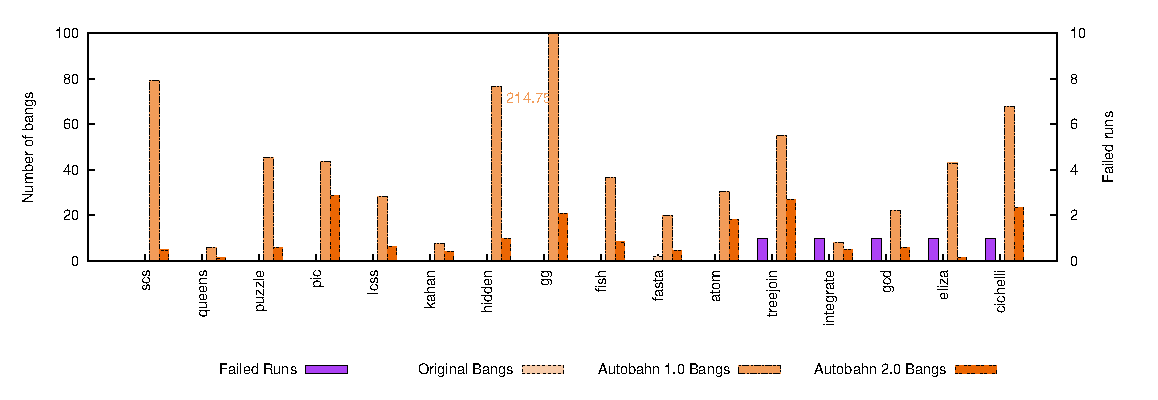
\includegraphics[width=\textwidth]{HA-bpapA}
\scaption{Number of bangs generated by \Ao{} vs. \At{} across the first
16 of 32 benchmarks that \At{} successfully optimized
at least once using memory allocations as the \profm{}. Failure
rate out of 10 runs is shown. Benchmarks are sorted in increasing order of
failure rate. Columns that exceed the maximum axis value are labeled
with their actual values.}
\label{fig:2-bangs-26-HA}
\end{figure*}

\begin{figure*}
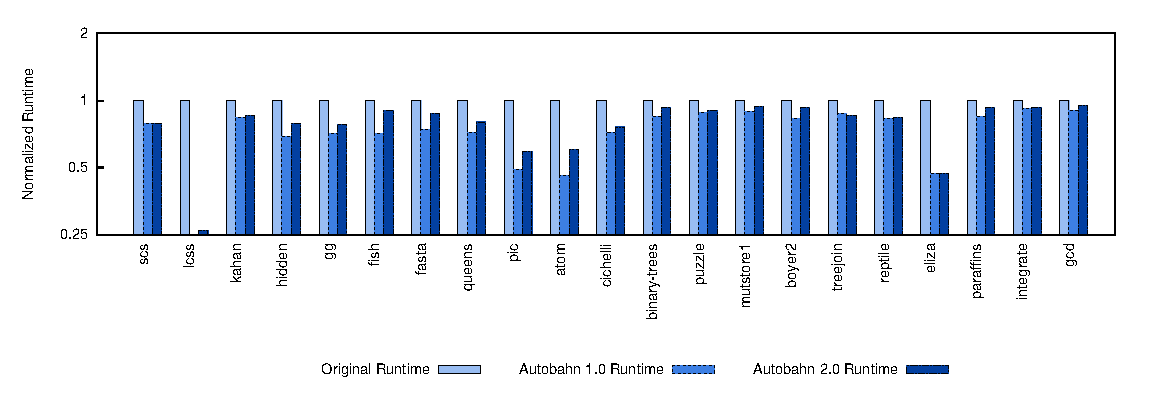
\includegraphics[width=\textwidth]{HA-papA}
\scaption{Runtime performance ratios of \Ao{} vs. \At{} across
the first 16 of 32 benchmarks that \At{} successfully optimized at least
once using memory allocations as the \profm{}. The x-axis is on a base-2 log scale.}
\label{fig:2-ratio-26-HA}
\end{figure*}

\begin{figure*}
\includegraphics[width=\textwidth]{HA-bpapb}
\scaption{Number of bangs generated by \Ao{} vs. \At{} across the remaining 
15 of 32 benchmarks that \At{} successfully optimized
at least once using memory allocations as the \profm{}. Failure
rate out of 10 runs is shown. Benchmarks are sorted in increasing order of
failure rate. Columns that exceed the maximum axis value are labeled
with their actual values.}
\label{fig:2-bangs-52-HA}
\end{figure*}

\begin{figure*}
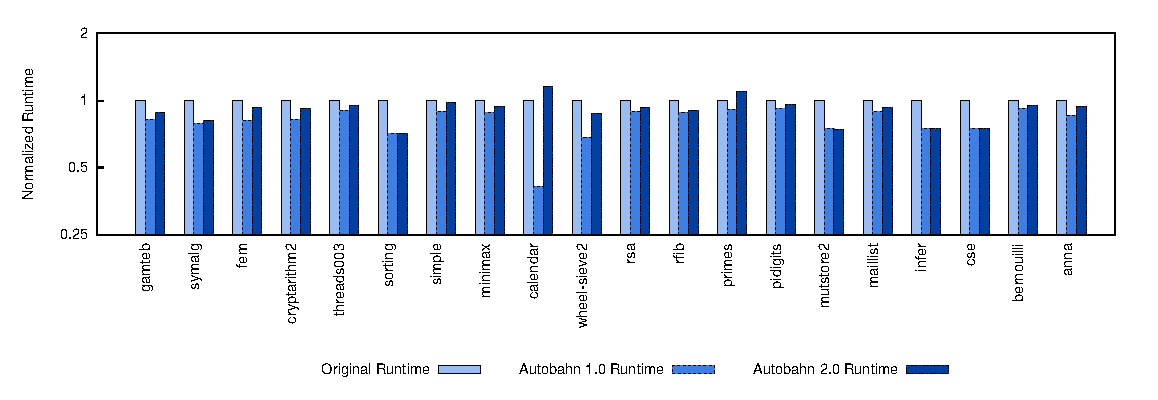
\includegraphics[width=\textwidth]{HA-papB}
\scaption{Runtime performance ratios of \Ao{} vs. \At{} across
the remaining 15 of 32 benchmarks that \At{} successfully optimized at least
once using memory allocations as the \profm{}. The x-axis is on a base-2 log scale.}
\label{fig:2-ratio-52-HA}
\end{figure*}


\begin{figure*}
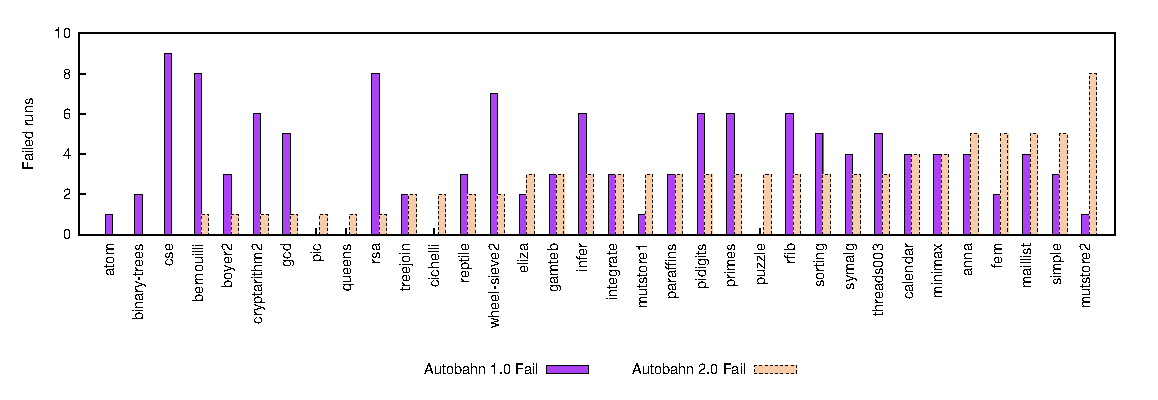
\includegraphics[width=\textwidth]{HA-pap-fail}
\scaption{Frequency of failure attributable to \Ao{} versus \At{} across the 45 
benchmarks that \At{} sometimes successfully optimized using memory allocations as the \profm{}. 
Benchmarks are sorted in increasing order of \At{} failure rate. }
\label{fig:failures-HA}
\end{figure*}

\begin{figure*}
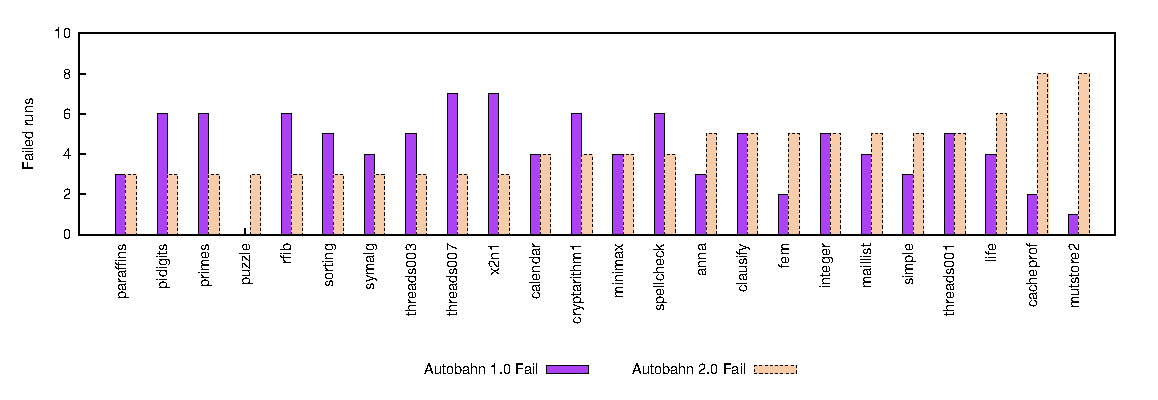
\includegraphics[width=\textwidth]{HA-pap-fail-2}
\scaption{Frequency of failure attributable to \Ao{} versus \At{} across the 45
benchmarks that \At{} sometimes successfully optimized using memory allocations as the \profm{}.
Benchmarks are sorted in increasing order of \At{} failure rate. }
\label{fig:2-failures-HA}
\end{figure*}

%----------------------------------------------------------------------------------------
%   SECTION 7
%----------------------------------------------------------------------------------------

\section{Case Study: \At{} On \texttt{gcSimulator}}
As a case study, we ran \At{} on \texttt{gcSimulator}, which is a
garbage collection simulator that consumes program execution traces
produced by the Elephant Tracks~\cite{Ricci13} monitoring system.  The
simulator comprises 2026~lines of code spread across 20~source code
files. To keep \Ao{} runtime within reasonable ranges, we used the
first 1M of the \texttt{batik} trace file from the DaCapo
benchmarks~\cite{Blackburn06} as the representative input.  For this
case study, we lowered the \absim{} threshold to 1\%
because \texttt{gcSimulator} does not have many \hotspots{} at higher
thresholds.  Once \At{} was done optimizing, we evaluated the
resulting program on larger trace file sizes of 100M and 500M. Because
running the simulator on the full 6184M trace size took too
long with or without optimization, we did not record results for the
full trace.

\Ao{} produces results that run
faster on representative input as well as on larger trace files.
\At{} was able to generate similar performance results with many fewer
bangs (125 vs. 690), as demonstrated in \figref{tab:gc}. 
While \figref{tab:gc} presents results from running \At{} using runtime
as the profiling metric, we also ran the same experiment using heap
allocations as the profiling metric. We did not find a significant
difference in using either profiling metric.

\begin{table}
\centering

\begin{tabular}{p{3cm}p{3cm}p{5cm}p{1.5cm}}
%\begin{tabular}{lllr}
\hline
Version   & File Size (M) & Runtime Performance Ratio& No.Bangs \\
\hline
Original      & 1       & 1         & 0   \\
              & 100     & 1         & 0 \\
              & 500     & 1         & 0 \\
\Ao{}         & 1       & 0.45      &  690\\
              & 100     & 0.33      &  690\\
              & 500     & 0.32      & 690\\
\At{}         & 1       &  0.58     & 125    \\
              & 100     & 0.37      & 125      \\
              & 500     & 0.38      & 125    \\

\hline
\end{tabular}
\scaption{Performance results for \texttt{gcSimulator}.}
\label{tab:gc}
\end{table}
